\section{Fixed-count ablation and sensitivity}
The selected two-group fits already hold cluster count constant. A second paired comparison fixes $k=3$ to ask whether enrichment reveals more useful structure at a moderately finer resolution.
\begin{table}[htbp]\centering\small
\caption{Paired K-means comparison at $k=3$. Common-space silhouette evaluates every assignment in the same standardized RFM coordinates; it tests preservation of RFM geometry, not a neutral measure of all possible usefulness.}\label{tab:fixed}
\begin{tabular}{lrrrr}\toprule
Space & Smallest group & Common RFM silhouette & Mean subsample ARI & Later $\eta^2$\\\midrule
RFM &397&0.357&0.970&0.313\\
Behavior &614&0.138&0.763&0.215\\
Product &677&0.079&0.929&0.170\\\bottomrule
\end{tabular}\end{table}
At three clusters, RFM retains stronger sampling reproducibility than either extension and explains a larger fraction of later-spend variance. Product is more stable than Behavior in this finer partition, but still offers no later-spend separation improvement over RFM. The paired bootstrap Product-minus-RFM difference in later $\eta^2$ is $-0.143$, with a conditional 95\% interval $[-0.165,-0.119]$. This is weaker stratification for the spending criterion. The common-space scores show that the enriched assignments depart from the baseline's geometry, as expected when the definition of similarity changes.

\begin{figure}[htbp]\centering
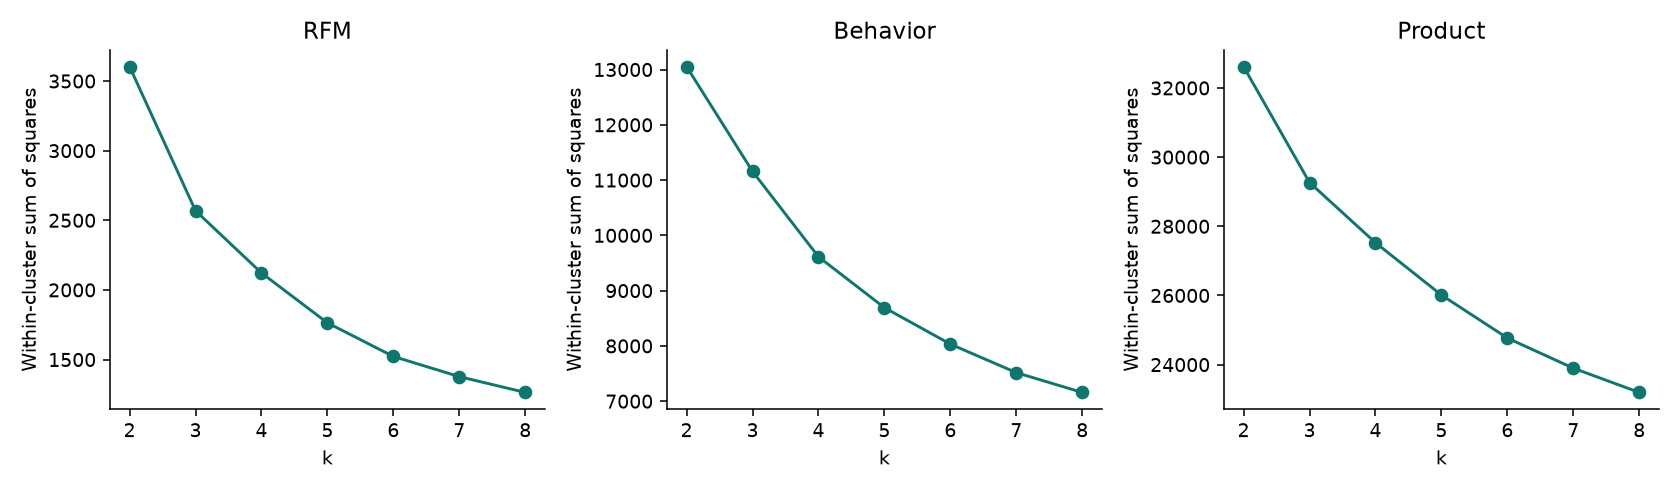
\includegraphics[width=\textwidth]{../figures/07_elbow.png}
\caption{K-means objective over the candidate cluster counts. Read each elbow within its own representation. Absolute inertia values across spaces have different scales and are not a ranking of model quality.}\label{fig:elbow}
\end{figure}
The Product representation's block weight is consequential. At fixed $k=3$, multiplying its category coordinates by 0.5 produces ARI 0.433 against the equal-block model; multiplying them by 2 produces ARI 0.460. Because variance scales with the square of a coordinate multiplier, these settings change the category block's variance to one quarter and four times its default. Such changes lead to materially different memberships even though all use the same data. An optimizer can reproducibly find an answer to a representation choice that remains debatable, so high repeated-start stability does not offset this sensitivity.


\begin{figure}[htbp]\centering
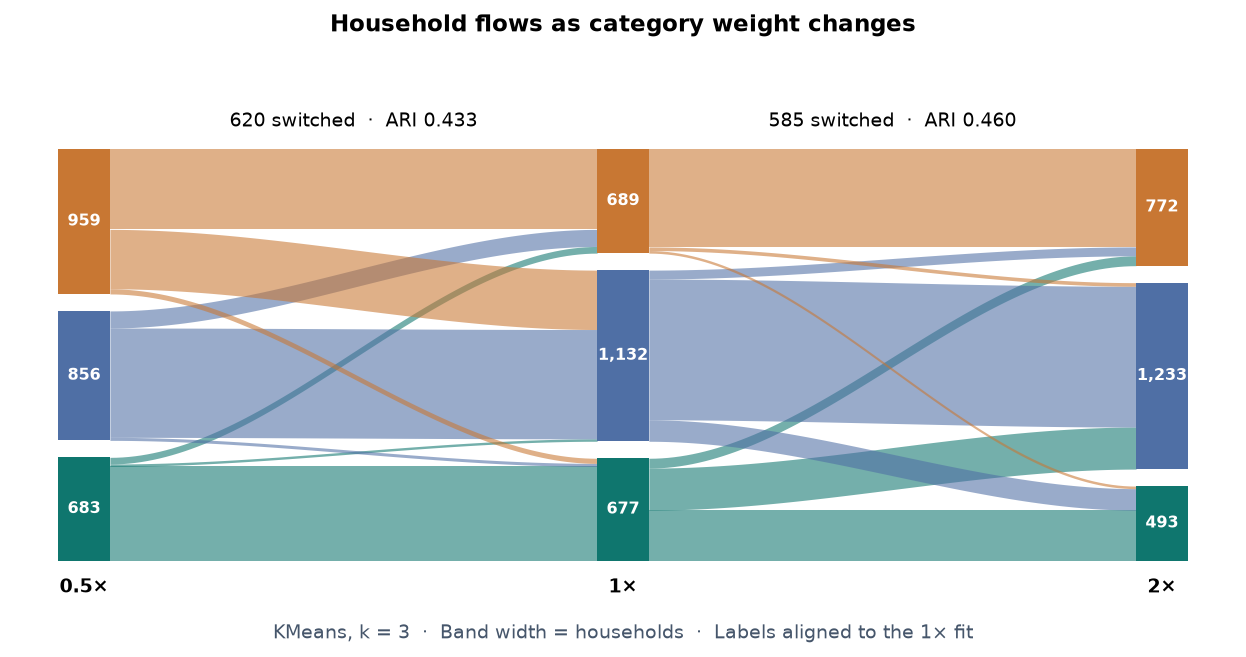
\includegraphics[width=\textwidth]{../figures/11_category_flow.png}
\caption{Household membership at three category-coordinate weights, holding $k=3$ fixed. Ribbon widths count households. Nondefault labels are matched to the default partition by maximum overlap; color is a visual correspondence, not a claim of identical cluster meaning. ARI remains invariant to label numbering.}\label{fig:flow}
\end{figure}
After maximum-overlap label alignment, halving the default category-coordinate weight changes 620 of 2,498 memberships (24.8\%), while doubling it changes 585 (23.4\%).

The flow view separates two questions: whether the optimizer repeatedly finds the same answer at a fixed weight, and whether that answer survives a different definition of similarity. Strong initialization stability answers the first question only. A practical segmentation should disclose the weighting choice and inspect the households affected by it.

\section{Practical interpretation and limitations}
\subsection{What the evidence supports}
RFM K-means with two groups is the best-performing model for this cohort. It is parsimonious, the most reproducible under household resampling (mean subsample ARI 0.980), and at least as informative for later spending separation as the enriched alternatives ($\eta^2=0.204$). The evidence supports two broad activity tiers rather than exactly two consumer types. Product-aware features add interpretable department descriptions and change household membership, but do not improve the principal diagnostics. The later-category check gives a small advantage (0.386\% versus 0.299\% of share variation explained) whose paired difference interval spans zero.

For a retailer, the practical implication is to use the RFM tiers for descriptive monitoring: compare assortment coverage, return activity and basket patterns between higher- and lower-activity households, and look for subgroups with unmet needs. Department profiles can supplement these tiers. Targeting decisions such as which coupon to send or which household to prioritize need an explicit objective and an experiment measuring incremental outcomes.

\subsection{Limitations}
The data are a historical panel from one retailer and do not capture total household grocery demand. Panel enrollment, incomplete observation, seasonality and store assortment may influence behavior, and the results may not generalize to current shoppers or another market. Positive-purchase filtering omits returns and zero-sales lines, so monetary features represent recorded buying activity rather than net margin. No observed later purchase does not prove defection.

Only one temporal split is examined. The 500-day calibration may blur changing preferences, and the 211-day holdout can have a different seasonal mix. Later spend favors historical spending features, so Product-aware groups might matter for a different objective, such as assortment breadth or category demand. All findings are observational and descriptive. The study does not estimate coupon responsiveness, campaign return, margin, customer lifetime value or causal marketing lift, and there is no independent ground truth or external replication.

The candidate grid is limited, DBSCAN tuning is exploratory, and only Euclidean K-means and Ward variants are tested. Correlated behavior features and category block weighting affect distances, and the $k=3$ check shows that weighting materially changes membership. Composition is coarse, with eight departments plus Other. Stability checks and bootstrap intervals condition on fixed preprocessing and fitted groups, and twenty resampling repetitions are a diagnostic rather than a population confidence interval. A PCA projection loses dimensions and is not proof of separability.

\subsection{Future improvements}
A stronger follow-up would predefine the retail decision and a relevance metric independent of feature development, repeat the analysis over rolling temporal origins, and refit the entire pipeline within resampling. It would compare multiple category resolutions and prespecified composition weights, extend the household case studies to systematic transition analysis, and monitor membership drift. A category-specific objective could show whether preference information adds value beyond intensity, and randomized trials would measure targeting benefits and costs.

\section{Conclusion}
\textbf{Main insights.} Adding basket behavior and department preferences to RFM does not improve household segmentation. All representative K-means fits select two broad activity groups, and K-means is more reproducible than Ward. The two groups separate recently active, high-frequency households from infrequent ones. Product features add department descriptions, but membership changes materially with category weighting (287 households change groups between RFM and Product). The exploratory later-category analysis shows some persistent profile differences, but no clear improvement over RFM in overall category-share separation. Coupon records that never entered clustering confirm the split: among households targeted by campaigns starting after day 500, 25.7\% of the RFM higher-activity group redeemed a coupon versus 4.8\% of the lower group, and Product labels do not separate responders better (Section~\ref{sec:extensions}).

\textbf{Best-performing model.} RFM K-means with $k=2$ performs best. It has the highest sampling stability (mean subsample ARI 0.980 versus 0.964 for Product) and the highest later-spend explained variance (0.204 versus 0.202). The fixed three-group comparison also favors RFM. It reaches these results with three features instead of seventeen.

\textbf{Business implications.} Use RFM tiers as the default for broad activity monitoring and treat department profiles as supplementary descriptions. For campaign planning, the four-group RFM persona view (loyal high-value, steady regulars, occasional shoppers and lapsed or at-risk households) re-slices the same activity gradient into actionable tiers: the loyal high-value group is 27.2\% of households but 56.6\% of later spend. A more complex segmentation is justified only for a validated category-specific objective.

\textbf{Limitations.} The data cover one retailer and one temporal split, and the findings are observational: they do not measure campaign lift or causal effects. Demographic data cover almost only higher-activity households, so they cannot profile the lower group.

\textbf{Future improvements.} Predefine the retail decision, repeat the analysis across rolling temporal origins, refit the full pipeline within resampling, test category resolutions and weights, and run randomized trials to measure targeting value.
